\chapter{Theoretical Part}

%%%%%%%%%%%%%%%%%%%%%%%%%%%%%%%%%%%%%%%
% PHYSICS
%%%%%%%%%%%%%%%%%%%%%%%%%%%%%%%%%%%%%%%
\section{Physical Background}\label{chapter:physics}

Before starting to ponder the structures of the human ear, it is necessary to understand the basics of how sounds work in the real world. It is safe to say that many people don’t ask this question – they just make sounds or react to them, unconsciously knowing the outcomes. Human mind has already developed a deep understanding of which sounds are produced under different circumstances – you can easily say what to expect when somebody scratches a blackboard or rings a bell. Some could say that sounds are just “pressure waves that propagate through the air”, but in reality, there is a lot of interesting and complex things beyond this definition to pay attention to. This section will introduce the reader to the underlying physics of sound and some interesting related concepts. A special focus will be made on describing harmonic sounds, which are essential to understand to be able to work with music and pitch.

\subsection{What a Sound Is}\label{section:physics_sound}

The definition of sound above, saying that it is just vibrations in the air, is hard to be called incorrect from the scientific point of view. Of course, there are improvements to be made: for example, that sound can propagate not only through the air, but through any medium that has inert mass and is “elastic”, or stiff, meaning that it will respond to forces applied to it. Making those corrections, it is also important to note that the definition above relates to sound as a physical phenomenon, but there is another definition that people use mostly in psychology and physiology, saying that the sound is a perception in the brain, or auditory sensation of the concept described above, or “an object of hearing”. It is possible to argue about the question of “What Is Sound?” for a long time, as people still haven’t come to a single definition and tend to mix the concepts \cite{Pasnau1999}, but in this thesis, the term “sound” will be used primarily in the first, physical sense, unless specified differently.\\

For better understanding of how physical sound works, keep in mind the mass and elasticity of the air mentioned above. Overall, mass and elasticity (not only of the air, but of any medium) play a very important role in the related studies: mass-spring systems are a highly discussed topic, along with the type of oscillations they tend to have. Any object that can produce sounds may be considered a mass-spring system: a bell, a guitar string, or even air or water, which can be thought of as many small masses connected by invisible springs\dots{} This knowledge is quite staggering -- in most cases, it is hard to imagine such system, because there could be no obvious mass nor elasticity. Consider an example for explaining resonant cavities: why a can of soda makes that clicking sound when it is being opened? The air is the answer. When you open the can, some parts of the air near its top act as a mass, and other parts near the bottom as a spring. The pressure in the can drops, and the “spring” at the bottom tries to suck the “mass” back in, producing the expected sound \cite{Schnupp2011}.\\

Now, if you imagine the simplest of such systems, like the one on figure \ref{img:vertical_mass_spring}, you can notice that when a particular force is applied to it, it tends to oscillate in a sinusoidal manner (due to some famous laws of physics, which will not be further discussed here). In fact, this can be applied to all mass-spring systems: they naturally “want” to vibrate in a sinusoidal fashion with a preferred frequency, called resonance frequency. Sinusoidal vibrations will be given more attention in chapter \ref{section:math_basics}.\\

\begin{figure}[t]
	\centering
	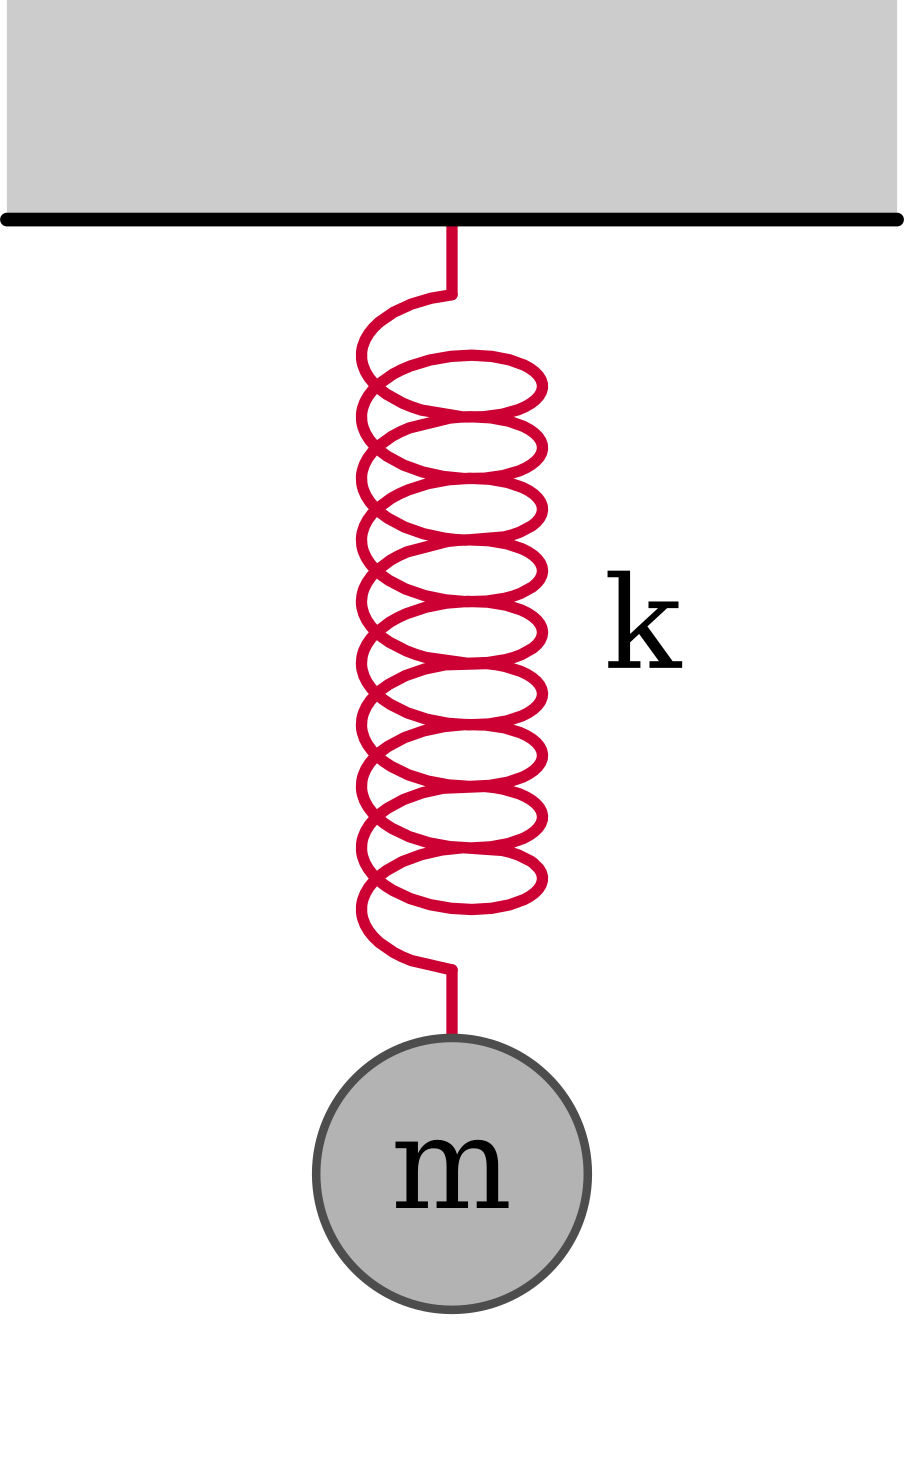
\includegraphics[height=0.25\textheight]{include/vertical_mass_spring}
	\caption[A simple vertical mass-spring system]{A simple vertical mass-spring system. Taken from \url{{https://commons.wikimedia.org/}}}
	\label{img:vertical_mass_spring}
\end{figure}

When someone talks about applying forces to objects, they can probably say that an impulse is delivered. In classical mechanics, impulse is a widely used concept, but for the purposes of this thesis, it is rather important to note how objects respond to impulses. When an impulse is delivered, the object starts to vibrate at all possible frequencies, but having in mind an understanding of resonance frequencies, it is safe to say that not all applied frequencies sound the same in the end. Thus, some tones in the resulting sound tend to be louder, and others, if not completely silent, highly attenuated. This frequency selectivity is based on the object's properties: the material of which it is made, its form, mass, \dots{} In signal processing, the notion of impulse response is widely used and will be referenced once again when discussing digital filters in chapter \ref{section:math_filters}. The above-mentioned “chosen” frequencies will be described a bit more in the next section.\\

Another essential topic to mention here is why sounds fade in time. This is again connected to the concept of mass-spring systems and the amplitudes of their vibrations. Usually, the greater these amplitudes are, the louder the resulting sound is, so if the amplitudes didn’t become smaller, we would live in constant unbearable noise. In brief, the fading is caused by the resistance of the medium, in which the sound propagates, and the manner of this propagating. It also depends on the material of which the sound source is made. If you imagine air as it was described above --- as many masses connected by invisible springs --- the mechanics of the propagation becomes clear: the sound source pushes the closest mass near it, which due to elasticity pushes its neighbors and returns to its starting location. Then its neighbors, in turn, push their neighbors and return, and so on, until these vibrations come to your ears. The air masses must be pushed again and again for the sound to spread, so it tends to lose its strength along the way, and the further from its source it travels, the smaller the amplitudes of the vibrations become.

\subsection{Harmonicity and Pitch}\label{section:physics_harmonics_pitch}

The conversation about how harmonics (or overtones) appear was already started in the previous section. In simple words, not all frequencies of the vibrations caused by delivering an impulse to an object keep their amplitudes for long. The ones that benefit the most from this phenomenon are harmonics, which are the periodic waves with frequencies that are positive integer multiplications of a specific frequency called fundamental (figure \ref{img:harmonics}). For example, if the fundamental frequency is 200\,Hz, the corresponding harmonics are 400\,Hz, 600\,Hz, 800\,Hz, 1\,kHz and so on. Each harmonic can be labeled with a number -- the fundamental frequency one is also called the 1st, so the wave with frequency of 1\,kHz from the example above would be the fifth. However, the scientific notation for harmonics might be confusing -- some authors refer to the fundamental frequency as $f_0$ (and the fifth harmonic would be $f_4$ in that case), others as $f_1$ (and $f_5$ respectively). In this thesis, fundamental frequency will be notated as $f_0$.\\

\begin{figure}[t]
	\centering
	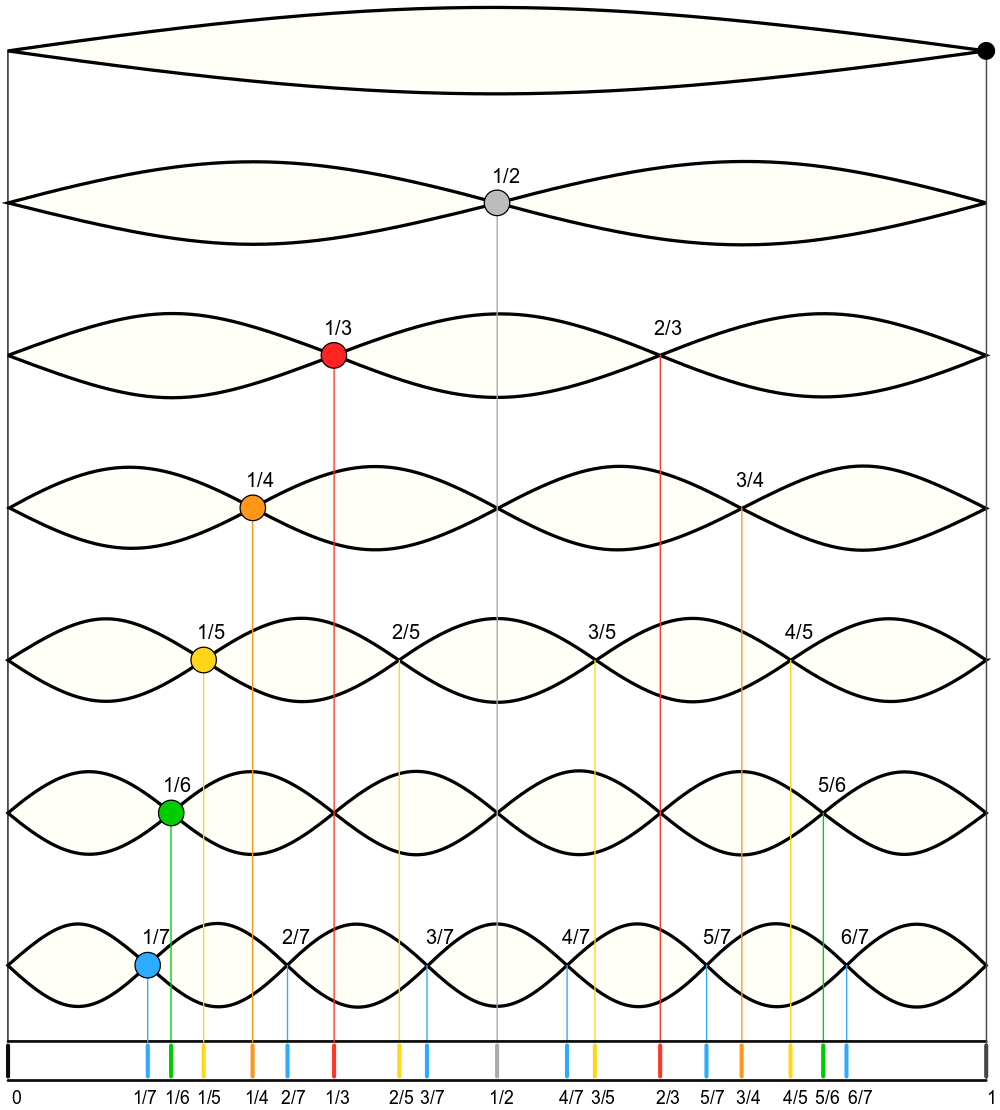
\includegraphics[width=0.6\textwidth]{include/harmonics}
	\caption[Harmonics of a sound wave]{First seven harmonics of a sound wave (or first seven modes of vibration of a string). Taken from \url{{https://commons.wikimedia.org/}}}
	\label{img:harmonics}
\end{figure}

Another explanation of how harmonics work might be found in \cite{Schnupp2011}. When you pluck a guitar string, it doesn't vibrate only as a whole. The same string might be thought of as two halves, or three thirds, or even one hundred one hundreds, and that each part of it vibrates separately. So, when the string is plucked, all its harmonics are excited, and the resulting sound is not a pure tone, but a complex one. This behavior is often called "modes of vibration" and might be observed not only in strings, but also, for example, in sheets of metal.\\

The most interesting property of harmonics is that they are all periodic at their fundamental frequency. If you sum up any number of adjacent harmonics of a wave, the period of the resulting wave would be equal to the period of the fundamental. This property plays an important role in the perception of pitch and is often used for its estimation in machine hearing systems.\\

Now, what is pitch exactly? To start using this term in the thesis, it is important to provide a clear definition, but in fact, there is none that is considered a standard. Two most widely used ones were given in \cite{Plack2005}. The first one was provided by the American Standards Association (ASA) in~1960 with a reference to music -- they defined pitch as \textit{"that attribute of auditory sensation in terms of which sounds may be ordered on a musical scale"} (\cite{Plack2005}, p.\,1). The second one was given by the American National Standards Institute (ANSI) in~1994 without a reference to music, saying that \textit{"Pitch [is] that attribute of auditory sensation in terms of which sounds may be ordered on a scale extending from low to high. Pitch depends primarily on the frequency content of the sound stimulus, but it also depends on the sound pressure and the waveform of the stimulus"} (\cite{Plack2005},~p.\,1). For this thesis, it is enough to consider pitch as the auditory sensation mentioned in both definitions that can be ordered on a scale.\\

It is important to note that pitch is not a physical property of sound, but perceptual. When someone says "low pitch" or "high pitch", it is not certainly clear where this "low" or "high" is -- low pitch for some people might be high for others. In the related studies of pitch perception in psychophysics, a term "just noticeable difference" (JND) is used, and there are references that humans can distinguish about 1\,400~points on the pitch scale.\\

Pitch is often associated with fundamental frequency, though it is not fully equivalent to it. Experiments have shown that for some short periodic sounds the perception of pitch might not appear at all, though it was clear that they had a fundamental frequency. On the other hand, there are reports saying that sounds with a missing fundamental (the ones made only from higher harmonics) could evoke the perception of pitch associated with the missing frequency, thus giving the illusion of what was not present in reality \cite{Schnupp2011}. Either way, pitch is a major attribute used while describing tones in Western music, as well as is loudness, duration and timbre. Pitch also plays an important role in auditory grouping, given the fact that same sound sources tend to produce sounds that are close in pitch. Auditory grouping in humans will be given more attention in chapter \ref{section:biology_asa}.

%%%%%%%%%%%%%%%%%%%%%%%%%%%%%%%%%%%%%%%
% BIOLOGY
%%%%%%%%%%%%%%%%%%%%%%%%%%%%%%%%%%%%%%%
\section{Biological Background}\label{chapter:biology}

Sounds are for sure one of the most important sources of information in our everyday life. By listening to them, one can describe what is happening around, understand how to react to occurring situations, or even tell if a danger is approaching, and it is time to take action. It is hard to imagine human sensation without hearing, but as easy as this may sound (no pun intended), the~biology behind it is quite complicated. This section will introduce the reader to how sound as a~mechanical phenomenon is converted to sound as perception and provide a~basic overview of the structures in the human ear, along with the mechanical and neurobiological processes happening inside of them.

\subsection{Outer and Middle Ear}

At the beginning, sound approaches the ear by vibrations in the air (or any other elastic medium) and enters the outer ear, which consists of the visible part (called the auricle, or the pinna) and the ear canal. The auricle is a thin plate of elastic cartilage, covered with integument, and connected to the surrounding parts by ligaments and muscles; and to the beginning of the ear canal by fibrous tissue. The ear canal is a tube leading from the~bottom of the~auricle to the middle ear, separated from it by the eardrum (or tympanic membrane). The main purpose of the ear canal is to focus the sound energy gathered by the auricle on the~eardrum. It also amplifies frequencies between 3\,kHz and 12\,kHz \cite{Standring2008}.\\

\begin{figure}[t]
	\centering
	\begin{subfigure}{0.5\textwidth}
		\centering
		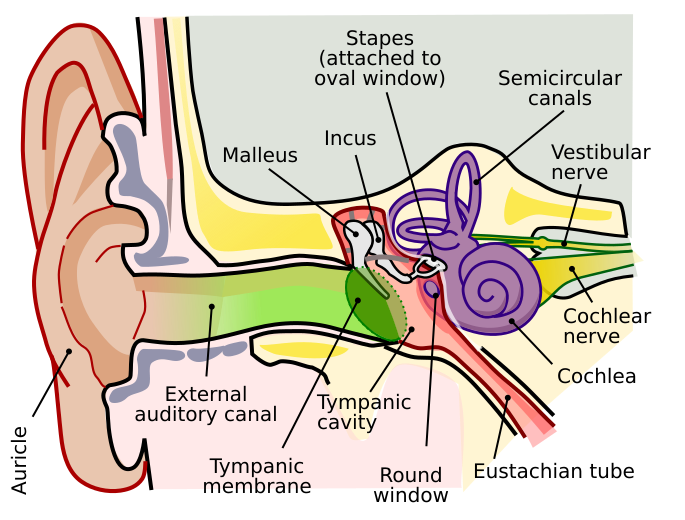
\includegraphics[width=\linewidth]{include/anatomy_of_the_human_ear}
		\caption{}
		\label{img:anatomy_human_ear}
	\end{subfigure}%
	\begin{subfigure}{0.5\textwidth}
		\centering
		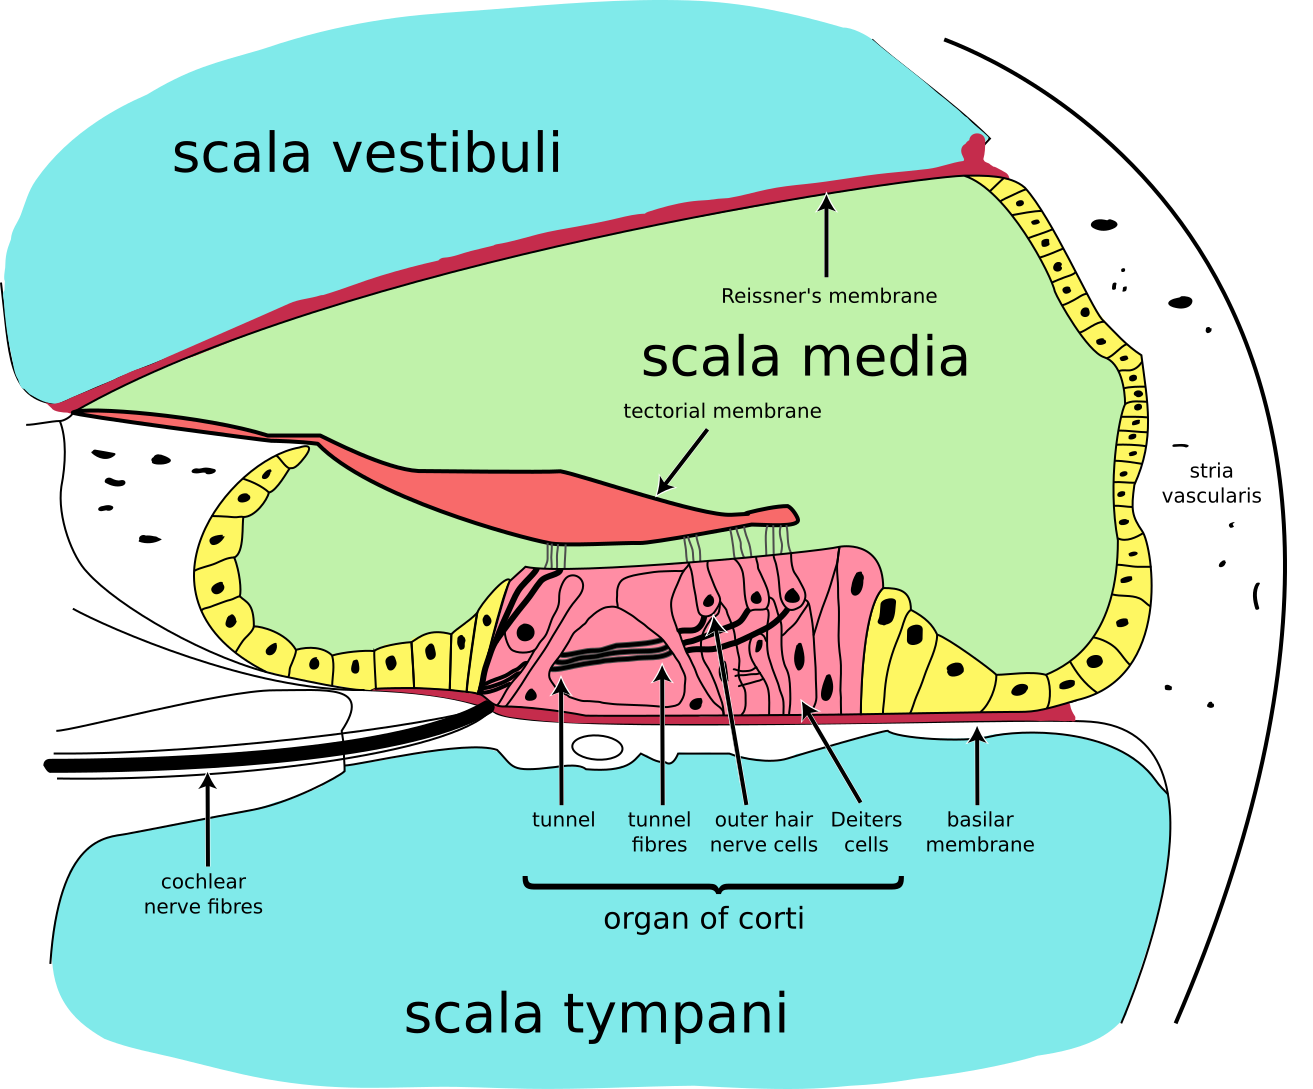
\includegraphics[width=\linewidth]{include/cochlea_cross_section}
		\caption{}
		\label{img:cochlea_cross_section}
	\end{subfigure}
	\caption[Anatomy of the human ear]{\textbf{(a)} Anatomy of the human ear. The ossicles of the middle ear are shown in white. The inner ear is shown in purple. \textbf{(b)} Cross-section of the cochlea showing the organ of Corti and three chambers filled with cochlear fluids. Both pictures were taken from \url{{https://commons.wikimedia.org/}}}
\end{figure}

Being gathered on the eardrum, the mechanical vibrations propagate through the middle ear. Three bones (called the ossicles) are located inside of it. The malleus (also called the hammer) is connected to the eardrum and transfers the vibrations from it to the incus (the anvil). These vibrations are chaotic, but the malleus is connected to the eardrum in a linear manner, helping the ear to respond more linearly and smoothly. The incus, in turn, connects to the stapes (the stirrup). The footplate of the stapes introduces pressure waves in the inner ear, which starts with the oval window of the cochlea. The structures of the middle ear can be seen on figure~\ref{img:anatomy_human_ear}.\\

It may sound redundant to have additional structures in the ear which propagate the vibrations even further, when they could travel just one centimeter more in a way like before, in the ear canal, but in reality, the pressure of these mechanical vibrations is too small to cause the waves of the same velocity in the cochlear fluids. The ossicles help to amplify the pressure of these vibrations. They are positioned to form a lever, and, because the oval window is about 14~times smaller than the eardrum, the pressure gain becomes quite significant in the end -- at~least 18.1~times \cite{Standring2008}.\\

To regulate the middle ear and protect it from damage due to very loud sounds, two muscles are located inside of it: the stapedius muscle and the tensor tympani muscle. These muscles are controlled by unconscious reflexes and hold the ossicles when the vibrations become too intense. To provide ventilation and drainage of the middle ear and to equalize pressures in this isolated environment, the middle ear is connected to the back of the throat by the eustachian tube \cite{Schnupp2011}.

\subsection{Inner Ear}

The inner ear starts with the above-mentioned oval window, which is connected to the stapes of the middle ear. The oval window is a part of the cochlea –- a structure of the inner ear dedicated to hearing. Along with the cochlea, the inner ear also contains the vestibular system, which is responsible for the sense of balance and spatial orientation and uses the same kinds of fluids and cells as the cochlea does. The vestibular system will not be covered in this thesis, but the fluids and cells will be described in more detail later in the section.\\

The cochlea itself is a spiral-shaped cavity made of bony tissue, which makes about 2.75~turns around its axis and is about 3\,cm long. The core component of it is the basilar membrane, which runs along almost its entire length and separates two of the three chambers of the cochlea filled with different fluids \cite{Schnupp2011}: the tympanic duct (scala tympani) filled with perilymph, and the cochlear duct (scala media) filled with endolymph. The third chamber, the vestibular duct (scala vestibuli), is separated from the cochlear duct by the Reissner’s membrane and is filled with perilymph (figure~\ref{img:cochlea_cross_section}). When the footplate of the stapes of the middle ear introduces movements to the cochlear fluids, the basilar membrane is affected too, and the endolymph in the cochlear duct moves along.\\

The most interesting property of the basilar membrane is that its stiffness and width is different throughout its length – the membrane is narrow and stiff at the basal end of the cochlea, and wide and floppy at the apical end. And here sound waves have two possible routes to take while propagating through the basilar membrane: a shorter path, which includes going through the stiffer parts of it, or a longer path, which means travelling along the membrane until it becomes easier to pass through, but pushing more fluid on the way. In fact, high-frequency waves tend to choose the shorter path, and low-frequency waves – the longer one. The distribution of frequencies passing through the basilar membrane is not linear, but close to logarithmic. In machine hearing systems, equivalent rectangular bandwidth (ERB) scale is usually used (see chapter \ref{section:math_concepts} for a definition).\\

Thus, the basilar membrane moves in different places depending on the frequencies of the vibrations. The organ of Corti, which sits on top of it and runs along its entire length, contains displacement cells able to detect movements of the fluid nearby and excite the nearby neurons to send electrical impulses. Such cells are packed with a bunch of stereocilia (hair) that stick out of its top, and thus are called hair cells. These cells can be of two types: inner hair cells that are located closer to the center of the cochlea, and outer hair cells that sit closer to its outer side. Inner hair cells are less numerous than outer hair cells and form a single row along the organ of Corti, while outer hair cells usually form three rows \cite{Schnupp2011}.\\

Now, it is important to mention that the endolymph in the cochlear duct contains high amounts of positively charged ions (primarily potassium and calcium). When it moves in response to the sound pressure, the stereocilia of the inner hair cells are deflected, and tiny ion channels open in them. This allows the charged ions from the endolymph to enter the stereocilia. The cell becomes depolarized, and a receptor potential is produced. This results in releasing the neurotransmitters at the basal end of the cell and then triggering action potentials in the nerve nearby. In this way, inner hair cells detect movements around them and convert mechanical sound waves to electrical nerve signals.\\

Outer hair cells, in turn, serve as amplifiers of the quiet sounds. Their receptor potentials are converted to cell body movements, thus increasing the sound pressure \cite{Hudspeth2008}.

\subsection{Auditory Scene Analysis}\label{section:biology_asa}

To close up the section, it was decided to make an introduction to auditory scene analysis according to Bregman \cite{Bregman1990}. His book named \textit{"Auditory Scene Analysis: The Perceptual Organization of Sound"} (1990) made a big influence on further researches, as it attempted to bring together the theoretical knowledge in the field that did not have any clear base to build on. Bregman's book is now widely recognized as this base, so it is necessary to list at least the primary concepts of ASA described there. This section could have been put to either of the chapters in the theoretical part of the thesis, because it is connected to every field being discussed, but it resides in the biological part, because most of the addressed experiments were testing human auditory perception and are highly connected to the related studies in Gestalt psychology.\\

To start off, Bregman brings to the world a new term related to auditory perception. If you recall the two definitions of sound from chapter \ref{section:physics_sound}, you may remember that there were two of them: one related to sound as a physical phenomenon, and another related to perception in the brain. Bregman introduced a term "auditory stream", or "auditory object", to address the second definition. He made an analogy with vision and how humans tend to group separate surfaces of the same object on their eye retina to see the object as a whole and referred to "auditory streams" as to the same kind of objects, but for audition. He said that the term "sound" is not really well suitable in this case, because for example a melody in a recording of music consists of different sounds (notes), but people often percept this melody as a whole and group the sounds into something greater in their perception. Bregman's definition of auditory streams became very popular, so it will be used throughout this thesis too.\\

Bregman defines ASA as the process of separating these auditory streams from mixtures and refers to it as to a two-stage process. The first stage (segmentation) is said to be splitting the auditory input into so-called "segments", just as the visible object is split into surfaces in the human eye. The second stage is grouping and refers to integrating the segments together based on the grouping cues. With references to experiments from his lab he describes two possible approaches to grouping and searching for cues: simultaneous (which is also called vertical, or spectral) and sequential (or horizontal). While simultaneous grouping takes into account the segments that appear at the same time, but relate to different frequencies (are spread in space), sequential grouping works with segments that share the frequency component, but are located at different points in time. As an example of a cue for simultaneous grouping one could take common onset and offset, because it is usual for sounds (or different frequency components of the same sound) from the same source to start at the same time. For sequential grouping, probably the most common cue is pitch. If two sounds have pitches associated with fundamental frequencies that are close to each other, the sounds will likely be grouped to the same stream. When the frequencies are further away, the sounds will most certainly appear in different streams.\\

For a demonstration of sequential grouping, consider a galloping sound that consists of two alternating tones: "A-B-A". The pattern repeats endlessly with a variable speed. The fundamental frequencies of the tones A and B can also be varied. Experimentally \cite{Schnupp2011} it was discovered that when the fundamental frequencies are close to each other and/or the speed of repeating the pattern is small, then there is only one resulting stream in the perception of the sequence. On the other hand, when the frequencies are further away and/or the sequence is being repeated at a faster rate, the subjects report that they can hear two streams: one consisting of repeating A-sounds ("A-{}-{}-A-A-{}-{}-A"), and another of repeating B-sounds ("-{}-B-{}-{}-{}-{}-B-{}-"). The subjects also reported that they can only focus their hearing only on one of the two streams, and the other one was heard in the background. Interestingly, when the repeating rate and the difference in frequencies were set to some specific values in between, the subjects reported that the perception of two streams was alternating with the perception of one stream every 15-20~seconds. This phenomenon was experimentally verified during the research for this thesis with the help of the website made for \cite{Schnupp2011}.\\

In his book \cite{Bregman1990}, Bregman described a similar experiment, but the repeating pattern was more complex. There were six tones: three lower ones (1,~2~and~3) and three higher ones (4,~5~and~6), and they were repeating in a pattern like this: "1-4-2-5-3-6". Bregman asked the subjects to report the order of the heard tones, and at faster rates of repeating they were failing to do this for both groups at the same time. When they were focusing the hearing on the lower tones, the higher ones were heard in the background, and thus it was difficult to correctly determine the order.\\

As an example for simultaneous grouping, Bregman makes another experiment. This time, the pattern consists of two alternating sounds: a pure tone (A) and a complex tone that consists of two pure tones (B and C). Again, the pattern repeats endlessly, and both the speed of repetition and fundamental frequencies of the tones might be changed. As a result, Bregman reports that the tone B was \textit{"an object of rivalry"} (\cite{Bregman1990}, p.654): in cases when A was close to it in frequency, they were grouped together in a simultaneous manner, but when they were further away from each other, the tone B was rather grouped simultaneously with C, thus creating a richer tone BC.\\

Bregman's theory is highly related to the studies in Gestalt psychology. He was drawing parallels between vision and hearing, and found a lot of similarities between them that were supported by the Gestalt laws of grouping. He described the concepts of "belongingness" and "exclusive allocation", and the principles of similarity, proximity and closure. Also, he was questioning whether scene analysis is an innate process, or the one acquired by learning.\\

Finally, to make a parallel with computer modeling, Bregman referred to the notion of heuristics. In his words, heuristics are \textit{"the procedures that are not guaranteed to solve the problem, but are likely to lead to a good solution"} (\cite{Bregman1990}, p.\,32). He believed that outputs from multiple heuristics should be used at the same time to find the good solution, and that there are similar mechanisms in human perception. For example, when there is evidence about common onsets and offsets of two frequency components of a sound, and it was supported by the fact that these components were different harmonics of the same fundamental frequency, the probability of being incorrect after guessing that these components should be grouped in the same stream becomes very close to zero. Here, two heuristics contributed to the decision of whether to group the sounds into a single stream.

%%%%%%%%%%%%%%%%%%%%%%%%%%%%%%%%%%%%%%%
% MATH
%%%%%%%%%%%%%%%%%%%%%%%%%%%%%%%%%%%%%%%
\section{Mathematical Background}\label{chapter:math}

Next, to address the practical part of the thesis, it is needed to give some attention to the underlying math. Considering that the system described in chapter \ref{chapter:implementation} extensively uses techniques and concepts from the field of digital signal processing, it was decided to make a brief introduction to the basics of it for a reader that might be confused by the variety of new terms. Thus, the present section will firstly describe how sounds are represented computationally, and then will provide a few examples of the most common ones. Next, a section dedicated to digital filters and filterbanks will follow, while other specific mathematical concepts used in the implementation part will be addressed later in chapter \ref{section:math_concepts}.

\subsection{The Basics of Digital Signal Processing}\label{section:math_basics}

As it was described in chapter \ref{section:physics_sound}, physical sounds in real world spread in the environment in a form of pressure waves. These waves are continuous, thus to be able to work with sounds via computers it is usually useful to convert them to some kind of a discrete representation. The notion of a discrete, or discrete-time, signal is used in these cases and is defined as a time series sampled at equally-spaced points on the time axis, or as a function of discrete time (for example, $x(n)$) \cite{Shenoi2005}. Digital signals are, in simple words, encoded representations of the discrete-time signals. The digital signal's sampling frequency $f_s$ is defined as a number of samples observed during a unit of time. Sometimes, digital signals are represented as vectors \cite{Abood2020}: \begin{equation}
	\textbf{x} = [x(0), x(1), \dots{}, x(N - 1)]^T\qquad\textbf{x}\in\mathbb{R}^N
\end{equation}
where $N$ is the overall number of samples.\\

If you recall the conversation about resonant frequencies and the sinusoidal manner of vibrations from chapter \ref{section:physics_sound}, you may remember that when an impulse is delivered to an object, the object responds to it by entering into vibrations. It starts to vibrate at all possible frequencies, but not all of them survive. An important mathematical instrument for frequency analysis is Fourier transform (along with Fourier series). Fourier theorem states that any periodic function might be represented as a sum of sines and cosines, so technically, any waveform of a sound (including the ones for sound waves) might be decomposed and represented in such a way. This decomposition may also be given by an amplitude spectrum and a phase spectrum \cite{Schnupp2011}.\\

The most basic example of such frequency decomposition is for a pure tone (the first row on figure \ref{img:windowing_example}). Pure tones are impossible to find in nature, or even perfectly produce with a speaker. Pure tones produced computationally sound flat and unnatural, but they are the basic building blocks of other sounds. The waveform of a pure tone is a sine wave and is defined as a function of time $t$:
\begin{equation}
	y(t) = a\sin(2\pi{}ft + \varphi)
\end{equation}
where $f$ is the frequency, $a$ is the amplitude and $\varphi$ is the phase. The frequency decomposition of a pure tone will contain only one peak at frequency $f$.\\

Another example of a common sound would be a click. Clicks are instant modulations in amplitude of a sound waveform, or waves that instantly go up and down at certain points in time. The most interesting fact about a click is its frequency decomposition being an infinite set of sine waves. More about clicks can be found, for example, in \cite{Schnupp2011}.\\

The last important sound that will be mentioned here is white noise. The waveform of a white noise is completely random, so its frequency decomposition is random too. White noise is used in the thesis for experiments with the resulting CASA system and its ability to separate music.\\

\begin{figure}[t]
	\centering
	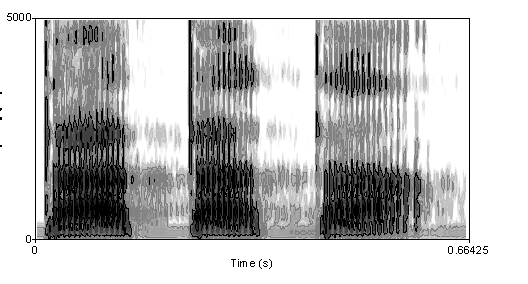
\includegraphics[height=0.25\textheight]{include/spectrogram_example}
	\caption[An example of a spectrogram]{A spectrogram of a male voice saying "ta-ta-ta". Time is shown on the horizontal axis, and frequencies are shown on vertical. The color intensity increases with density. Three separate syllables are clearly visible. Taken from \url{{https://commons.wikimedia.org/}}}
	\label{img:spectrogram_example}
\end{figure}

Continuing the conversation about frequency decomposition, it is necessary to note that it is impossible to extract any information about the time component from the output of the Fourier transform. Thus, it is useful to firstly split the wave into separate intervals on the time axis (which are often called windows), and only then compute their frequency decompositions. The resulting time-frequency representation of the sound wave is called spectrogram. An example of a spectrogram is shown on figure \ref{img:spectrogram_example}.\\

However, there is a known problem that emerges when windowing is used with the Fourier transform. When the window is rectangular (the wave is cut off vertically from both sides) and is not aligned with the period of the signal, the onset and offset of the wave become abrupt. These sudden changes in amplitude result in the necessity of adding countless additional sine waves to the frequency decomposition, and it begins to contain chaotic information, which makes the valuable parts of the spectrum less precise. An example of this behavior was given in \cite{Schnupp2011} and is shown on the second row of figure~\ref{img:windowing_example}.\\

A viable solution of this discontinuity problem comes with attempts to smooth the abrupt ends of the masked wave. Windows that have some kind of ramping on both sides are used in this case. The ramping helps to smoothly turn the sound on and off and reduce the "spectral splatter" \cite{Schnupp2011}. An example of such window (Hanning window) is shown on the third row of fi\-gure~\ref{img:windowing_example}.\\

\begin{figure}[t]
	\centering
	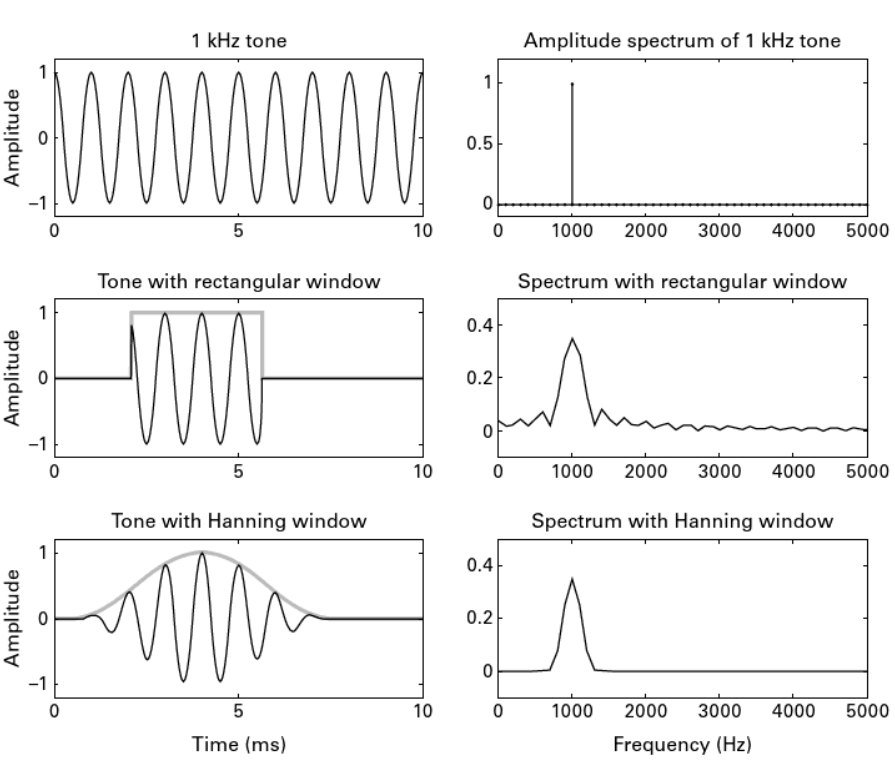
\includegraphics[width=0.75\textwidth]{include/windowing_example}
	\caption[An example of windowing and the problem of discontinuities]{The problem of discontinuities that arises when rectangular windows are used. The first row depicts a 1\,kHz pure tone (a sine wave) and its amplitude spectrum. The second row demonstrates the amplitude spectrum of the same tone masked by a rectangular window. The third row shows the spectrum of the same tone masked by a Hanning window. The window functions are shown in gray. Taken from \cite{Schnupp2011}.}
	\label{img:windowing_example}
\end{figure}

It is also worth noting that when the masking window is short, the resulting amplitude spectrum becomes wider, and vice versa: when the precise frequency representation is needed, the time window must be wide enough. This property is called time-frequency trade-off and can be observed in spectrograms: the spectrograms with high frequency resolution usually have low time resolution, and the ones with high time resolution have low frequency resolution.

\subsection{Filters and Filterbanks}\label{section:math_filters}

In chapter \ref{section:physics_sound}, when there was a conversation about the objects' impulse responses, some attention was given to the selectivity of frequencies. It was said that frequencies that don't align with the object's resonance frequency are attenuated, or filtered out. Thus, the mentioned object might be thought of as a mechanical linear filter. The linearity comes from the fact that the force applied to the object is proportional to the amplitude of the output signal (in simple words, the harder you pluck the guitar string, the louder the resulting sound will be). The linear filter's impulse response is a function of time that depicts how it responds to a simple external impulse, and its frequency response is a function that shows how much different frequencies are affected after the filtering.\\

The filters used in the implementation part of the thesis are digital, meaning that they ope\-rate on discrete-time or digital signals by performing different mathematical operations. Their counterpart is analog filters operating on continuous-time (also called analog) signals \cite{Shenoi2005}. Linear filters might be of two types: infinite impulse response (IIR) or finite impulse response (FIR). Impulse response of an IIR filter does not become equal to zero after a certain point in time, but continues infinitely, whereas impulse response of an FIR filter is given only for a certain time interval. FIR filters are usually non-recursive and less efficient, while IIR filters are recursive and computationally better.\\

The technique that is used for filtering of signals is called convolution. For digital signals, it is defined as follows \cite{Schnupp2011}:
\begin{equation}
	(f*g)(n) = \sum_{m=0}^{N-1}f(m)g(n - m) = \sum_{m=0}^{N-1}f(n - m)g(m)
\end{equation}
where $f(n)$ is the input signal, $g(n)$ is the filter impulse response, $m$ is the delay, or lag, and $N$ is the overall number of samples. Convolution is commutative, thus the functions for the input signal and the filter impulse response may be swapped.\\

The last term for this section is a filterbank. Basically, a filterbank is a collection of filters with different properties. In the implementation part, a filterbank of gammatone filters is used to simulate the basilar membrane of the human inner ear.

%%%%%%%%%%%%%%%%%%%%%%%%%%%%%%%%%%%%%%%
% CASA
%%%%%%%%%%%%%%%%%%%%%%%%%%%%%%%%%%%%%%%
\section{Computational ASA}\label{chapter:casa}

Now, having described the underlying concepts from different fields of science in previous sections, it is time to finally focus on computational auditory scene analysis. CASA is said to be the study that groups practical, programmable solutions for auditory scene analysis problems, or the study of ASA by computational means. CASA systems are used primarily for source se\-pa\-ra\-tion, meaning that they are machine listening systems that aim to separate "target" sounds from mixtures, just like people do when try to focus on a specific sound and not to be distracted by others. In that CASA systems differ from systems for blind signal separation – they try to mimic (at least to some extent) the mechanisms inside the human ear, which were discussed in chapter~\ref{chapter:biology}. In this chapter, main principles of CASA systems will be described, along with a typical architecture, goals and applications. In the second part, major works that use computational auditory scene analysis for source separation will be reviewed and compared.

\subsection{Principles, Goals and Applications}

Having the definition of CASA above, to be able to limit the requirements to the models it is necessary to describe the principles of CASA and common concepts across different systems. As the most major one, one could pick the restriction of number of microphones used in the input. Being based on the mechanisms of the human auditory system, CASA models only use recordings from one or two microphones (to simulate one or two ears), thus being split to monaural and binaural. Monaural models are researched better, but can't be used for extracting features based on the location of the sound, which is possible to some extent in binaural models, when time differences between the two recordings might be used.\\

To discuss the goals of CASA, it is useful to refer to the goals of ASA. According to Bregman~\cite{Bregman1990}, the primary goal of auditory scene analysis is to produce separate streams from the auditory input. Here, the term "stream" refers to a representation of a distinct sound source in the acoustic environment (see chapter \ref{section:biology_asa}), but, for example in \cite{Wang2006}, the authors also use it when talking about these representations in computer memory.\\

For CASA, Wang and colleagues \cite{Wang2005} proposed that the goal should be to find an ideal binary mask (IBM) for the time-frequency (T-F) representation of the input. If the input is split into T-F units, where time is on horizontal axis and frequency on vertical, the IBM is a binary matrix that has ones in places where the target sound is stronger, and zeroes elsewhere for background units. Ideal binary masks (and time-frequency masks overall) will be given some more attention in chapter \ref{subsection:casa_segmentation_and_grouping}.\\

The research of CASA systems and their applications in science \cite{Szabo2016} has been quite diverse recently. Some of the models are inspired by various biological experiments \cite{Wang2008}\cite{Boes2011}, while others are trying to address the cocktail party problem in natural environments \cite{Elhilali2008}. Some models try to explicitly simulate perceptual data, but others may refer to perception only very slightly. The expected output for the system implemented in this thesis is to find an IBM to be able to mask noisy background in monophonic piano music.\\

Aside from pure scientific interest, CASA systems find useful applications in everyday life \cite{Wang2006}. Some of them are listed below.

\begin{description}
	\item[Speech recognition] Apparently, speech recognition is the most popular field, where CASA systems have been used. Many speech recognition systems have performance losses in acoustic environments, where multiple sources of sound are present. The development is often put in contrast with computer vision systems that basically fulfill the same purpose, but for another human sense.
	\item[Automatic music transcription] A complex problem on its own (even human experts can come up with different solutions) becomes more complicated when multiple musical instruments are involved and need to be transcribed separately. CASA can certainly bring new insights to the field.
	\item[Hearing prostheses] Modern hearing aids made for people suffering from hearing loss don't separate speech in noisy environments, amplifying the noisy background too. CASA could address this problem to filter the noise out at least to some extent.
	\item[Audio information retrieval] Recordings on the Internet usually contain mixtures of sounds from different sources, thus it is necessary to separate them to be able to search efficiently.
\end{description}

\subsection{Major Works}

